\begin{figure}[t]
\centering
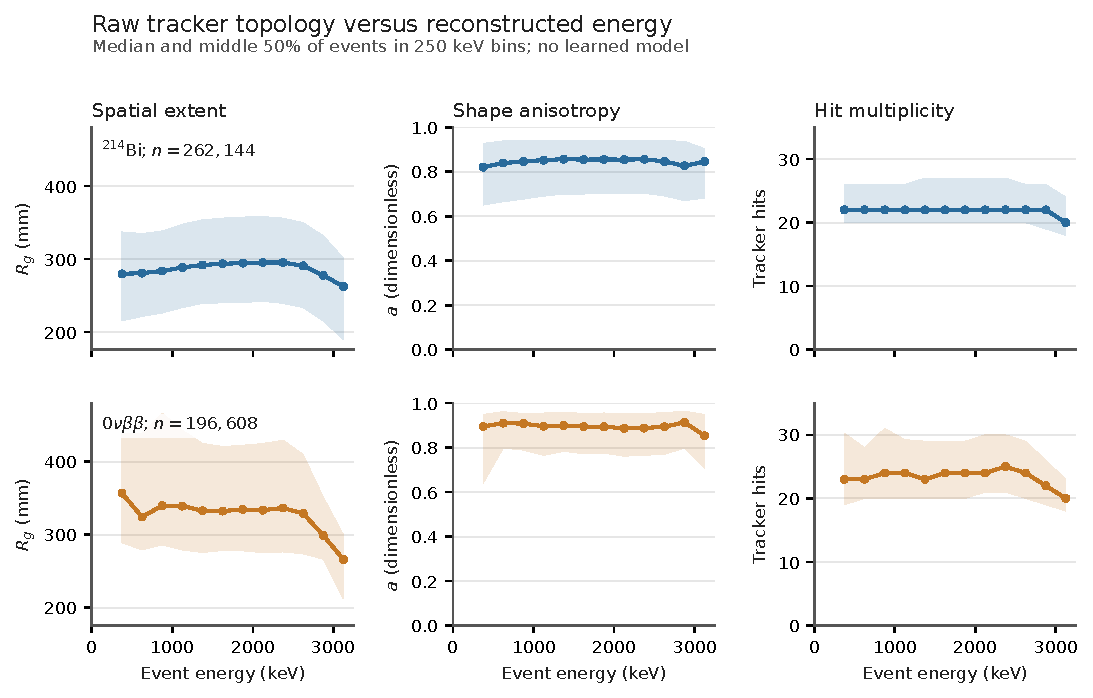
\includegraphics[width=\linewidth]{wing_contribution/figures/supernemo_geometry_energy.pdf}
\caption{Raw tracker topology as a function of reconstructed calorimeter
energy, compared within each physical class. Radius of gyration measures
spatial spread, anisotropy measures elongation, and hit count measures
observed multiplicity. Points mark medians and shaded regions contain
the middle 50\% of events in fixed 250\,keV bins, with all 262,144
$^{214}$Bi and 196,608 $0\nu\beta\beta$ test events included. Lines connect
bin summaries rather than fit a model. The shading is not a confidence
interval. Exact
definitions and event-level checks are given in
Appendix~\ref{app:raw-observations}. No learned model or energy-matching
weights enter this diagnostic.}
\label{fig:geometry-energy}
\end{figure}
